\section{Optimizations}\label{sec:optim}

\fixme{Manoj and Sharmila holds the lock}
\subsection{Optimizations for Scan Window Processing}
\begin{itemize}

\enumerate{Using Shared Memory:}
Information about the classifiers as mentioned in Section
\ref{sec:haar} are common to all the scan windows. Hence the first optimization 
is to bring the data related to classifiers. But since there are 2913 classifiers 
for the entire face detection process, it requires 209.836kB of storage for the data. 
But a maximum of 48kB shared memory is available. Hence we split the scan window processing 
into multiple kernels with n stages in each kernel that correspond to around 320 Haar classifiers. 
This requires 12 kernels with around 19kB of shared memory each.
Using Pinned Host Memory: When allocating memory on CPU for the data that needs to be transferred 
to GPU, there are two types of memory to choose from: \emph{Pinned} and \emph{Non-Pinned}. 
Pinned memory is not swapped out from the memory by the OS for any reason and hence provides 
improved transfer speeds. CUDA provides \emph{cudaMallocHost} API that can be used instead of 
usual \emph{malloc} to achieve this.

\enumerate{Using Fast Math:}
Our algorithm makes use of calculating standard deviation which is the square 
root of variance. If we make use of \emph{-use\_fast\_math} flag while compiling using \emph{nvcc}, 
we explicitly instruct GPU to use its Special Functional Unit to calculate square root. This provides 
lesser precision but at a greater speed. 

\enumerate{Not using restriction on maximum registers per thread:}
In our baseline implementation, we had 
restricted maximum register count per thread to 20 to increase occupancy. But scanning window 
kernel requires 28 registers. Because of the restriction there was spilling of registers that 
increased the execution time. Hence we removed the imposition and observed decreased execution 
time even though occupancy decreased. This showed occupancy is not always a measure of performance.

\enumerate{Using block divergence:}
In the baseline implementation, each thread continued execution up to 25 stages 
even if the scan window failed any previous stage. Rejecting a thread as early as possible leads to thread 
divergence that leads to under-utilization as in Figure~\ref{fig:tdiv}. But if all the threads in a block 
are rejected, block divergence occurs and the entire block will not be launched at all thus increasing 
performance as in Figure~\ref{fig:bdiv}. Since each kernel can consist of multiple stages, we reject a 
scan window at kernel-level granularity. Images that have one or two faces have only few scan windows that 
have face. Using this optimization, we have made the common case faster. Hence according to 
\emph{Amdahl’s law} we observe huge increase in performance. 

\begin{figure}[h]
  \centering 
  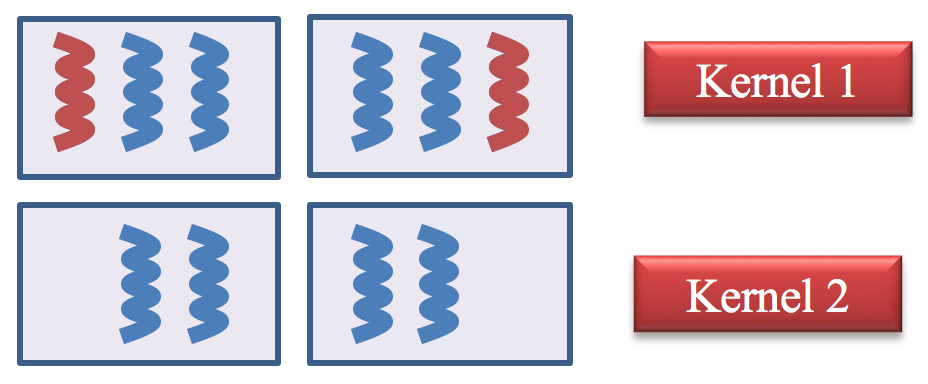
\includegraphics[width=\linewidth]{figs/thread_div.jpg}
  \caption{Example of Thread Divergence \textnormal{\small }  }
  \label{fig:tdiv}
\end{figure}


\begin{figure}[h]
  \centering 
  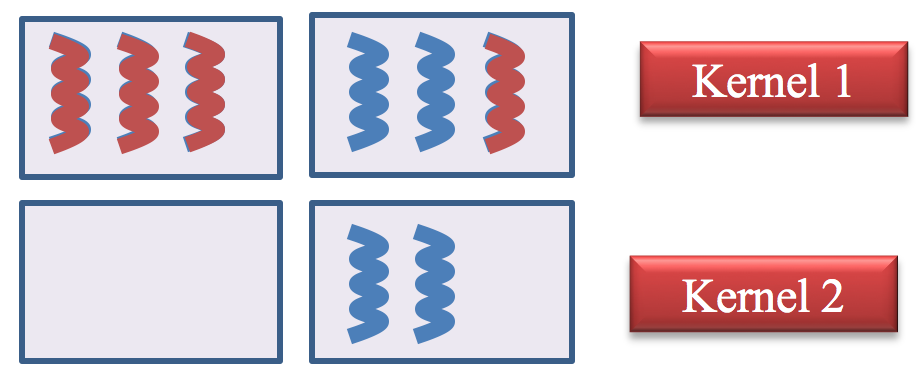
\includegraphics[width=\linewidth]{figs/block_div.jpg}
  \caption{Example of Block Divergence \textnormal{\small }  }
  \label{fig:bdiv}
\end{figure}


